% Licensed under the Creative Commons Attribution Share Alike 4.0 International.
% See the LICENSE file in the repository root for full license text.

\section{通过命令行使用 CMake}

虽然我本人更喜欢使用图形化界面,但是在某些时候,我们只能使用\emph{命令行(command line)}:比如\emph{持续集成(continuous integration, CI)}系统只允许你编写命令行形式的脚本程序,亦或是远程连接的服务器只能通过\emph{终端(terminal)}访问。本节将简要介绍通过命令行使用 CMake 配置项目、生成程序的方法。

仍然以 Windows 操作系统为例。读者可以使用命令提示符、Powershell 等终端。直接在终端中输入 \lstinline[language={}]{cmake},即可看到图 \ref{fig:cmd-1} 所示的内容。如果你收到了类似于“无法找到程序”的错误信息,请检查在安装 CMake 时是否像图 \ref{fig:cmake-installment} 一样将 CMake 添加到了 PATH 环境变量中。

\begin{figure}[H]
	\centering
	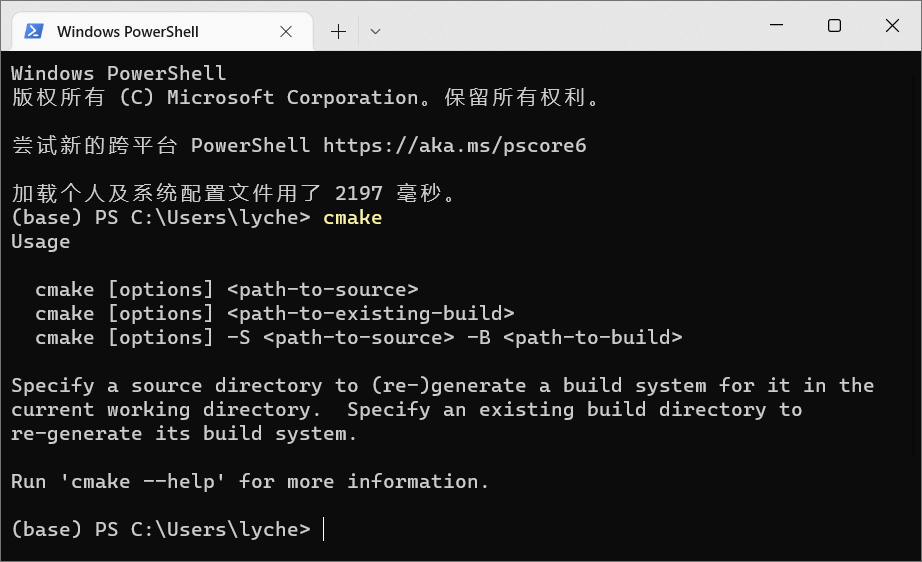
\includegraphics[width=0.8\linewidth]{assets/cmd-1}
	\caption{在命令行中直接输入 \lstinline[language={}]{cmake} 后的结果。}
	\label{fig:cmd-1}
\end{figure}

图 \ref{fig:cmd-1} 告诉了我们一个重要信息:与其他所有命令行程序一样,可以输入 \lstinline[language={}]{--help} 选项查看帮助信息。\lstinline[language={}]{cmake --help} 命令的执行结果如图 \ref{fig:cmd-2} 所示。
我们不会在本节中介绍这些选项,我们接下来只简单介绍如何\emph{配置项目(configure)}和\emph{生成程序(build)},其余的少量内容将在之后需要时讲解,剩下的绝大部分内容都应该根据需要自学。

\begin{figure}
	\centering
	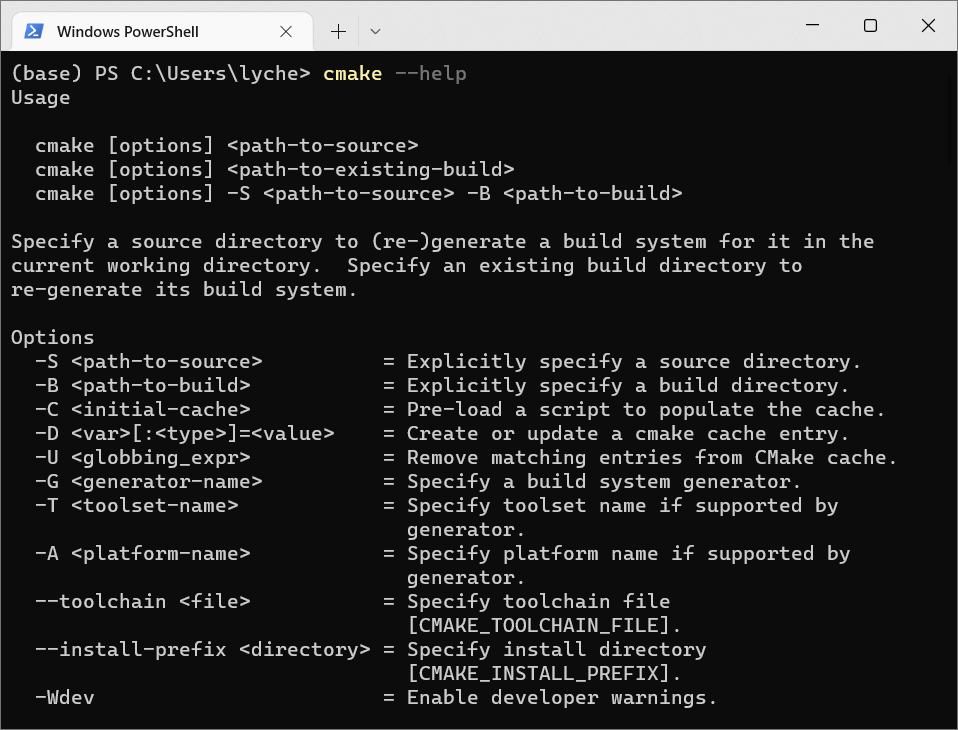
\includegraphics[width=0.8\linewidth]{assets/cmd-2}
	\caption{在命令行中输入 \lstinline[language={}]{cmake --help} 后的结果。}
	\label{fig:cmd-2}
\end{figure}
